\section{Durchführung}
\label{sec:Durchführung}
\subsection{Versuchsaufbau}
\begin{figure}[h]
    \centering
    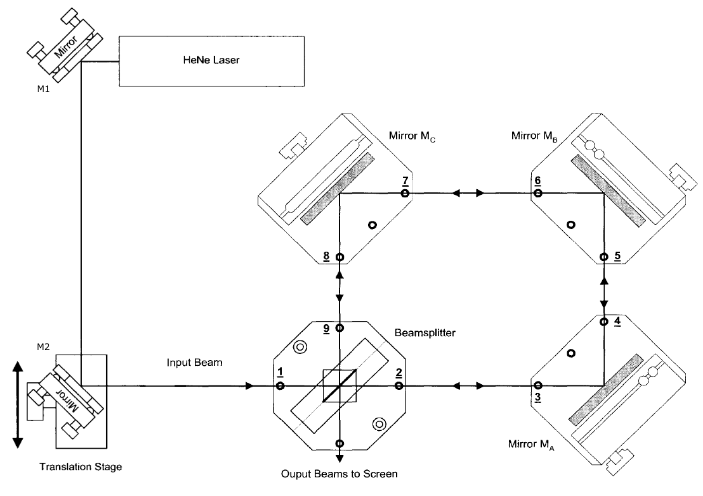
\includegraphics[width = \textwidth]{bild/Aufbau.png}
    \caption{Eine Darstellung des Versuchsaufbaus, der aus einem Sagnac-Interferometer besteht \cite{V64}.}
    \label{fig:Aufbau}
\end{figure}

\noindent
Der Versuch besteht aus einem Sagnac-Interferometer~\ref{fig:Aufbau},
in das ein Laser mit der Wellenlänge \SI{632.990}{\nano\metre} gestrahlt wird. 
Vor dem Interferometer steht ein Polarisationsfilter im Strahlgang.
Der Strahl trifft nach dem Verlassen des Interferometers auf einen 
\textit{polarizing beam splitter cube} (PBSC), 
der diesen in seine vertikale und horizontale Polarisationskomponente zerlegt,
wodurch die Strahlen eine Phasenverschiebung von 180° haben.
Diese werden auf zwei Dioden geleitet,
mit denen die Differenz der Photodiodenspannungen gemessen 
und auf dem Oszilloskop angezeigt wird.

\subsection{Justierung}%%%%%%%%%%%%%%%%%%%%%%%%%%%%%%%%%%%%%%%%%%%%%%%%%%%%%%%%%%%%%%%%%5555
Zuerst wird das Sagnac-Interferometer justiert,
sodass die den Strahlen parallel zueinander verlaufen.
Dazu werden die Justierplatten auf Position 1 und 3 gestellt 
und der Strahl über Spiegel $M_1$ und $M_2$ durch das mittlere Loch der Platten gestrahlt.
Der reflektierte Strahl wird abgeschirmt.
Die werden Justierplatten auf Postition 8 und 9 gesteckt und
der transmitierte Strahl über Spiegel $M_A$ und $M_C$  justiert.
Mit den Justierplatten auf Position 4 und 7 wird Spiegel $M_B$ eingestellt.
Die Strahlen werden über den Spiegel $M_2$ getrennt.
\noindent Ist alles korregt justiert,
sind die Strahlen nach dem Verlassen des Interferometers parallel und
treffen in einem Punkt auf den Schirm.
Bei konstruktiver Interferenz hat dieser Punkt seine maximale Helligkeit 
und bei destruktiver Interferenz verschwindet er.
Liegen die Strahlen nicht genau übereinander, sind Streifen zu sehen
und können über die Spiegel feinjustiert werden.

\subsection{Kontrastbestimmung}%%%%%%%%%%%%%%%%%%%%%%%%%%%%%%%%%%%%%%%%%%%%%%%%%%%%%%%%%%%%%%%%%%%%%%%%%%%%%%%%
Der Kontrast wird in Abhängigkeit der Polarisation gemessen,
indem vor dem Strahlteiler ein Polarisationsfilter gestellt wird.
Die Intensität der Interferenzmaxima/-minima wird für verschiedene Polarisationswinkel gemessen.
\newline \newline
\noindent Für die weiteren Messungen wird der größte Kontrast eingestellt.

\subsection{Messung des Brechungsindex von Glas}%%%%%%%%%%%%%%%%%%%%%%%%%%%%%%%%%%%%%%%%%%%%%%%%%%%%
Zwei Glasplatten werden mit einem Winkel von $10°$ 
in die parallel laufenden Strahlen gestellt.
Die Platten werdem um $10°$ gedreht und die Anzahl der Interferenzminima  oder -maxima bestimmt.
Diese Messung wird insgesamt 10 mal wiederholt.

\subsection{Messung des Brechungsindex von Luft}%%%%%%%%%%%%%%%%%%%%%%%%%%%%%%%%%%%%%%%%%%%%%%%%%%%%%%%%%%%%%%%%%%%%%%%%%%%%%%%%%%%%%%%%%%%%%%%%%%%%%%%%%%%%%%%%%%%%%%%%%%%%%%%%%%%5
In einen der Strahlen wird eine evakuierte Gaszelle gestellt.
In 50 mbar-Schritten wird der Druck erhöht, bis wieder der Normaldruck erreicht ist.
Währenddessen wird die Anzahl der Interferenzmaxima notiert.
Die Messung wird 3 mal durchgeführt.
